% ============================================================
%  CAPITOLO 3 --- PROGETTAZIONE CONCETTUALE
% ============================================================
\chapter{Progettazione concettuale}

In questo capitolo si descrive lo sviluppo dello schema Entit\`{a}-Relazione (E/R).
La progettazione procede per raffinamenti successivi, partendo da uno schema scheletro
e arricchendolo progressivamente per area tematica.

% -- 3.1 Schemi scheletro ------------------------------------
\section{Area Ordini}

\subsection{Schema Scheletro}
\begin{figure}[H]
  \centering
  % -- Inserire qui l'immagine dello schema scheletro ------
  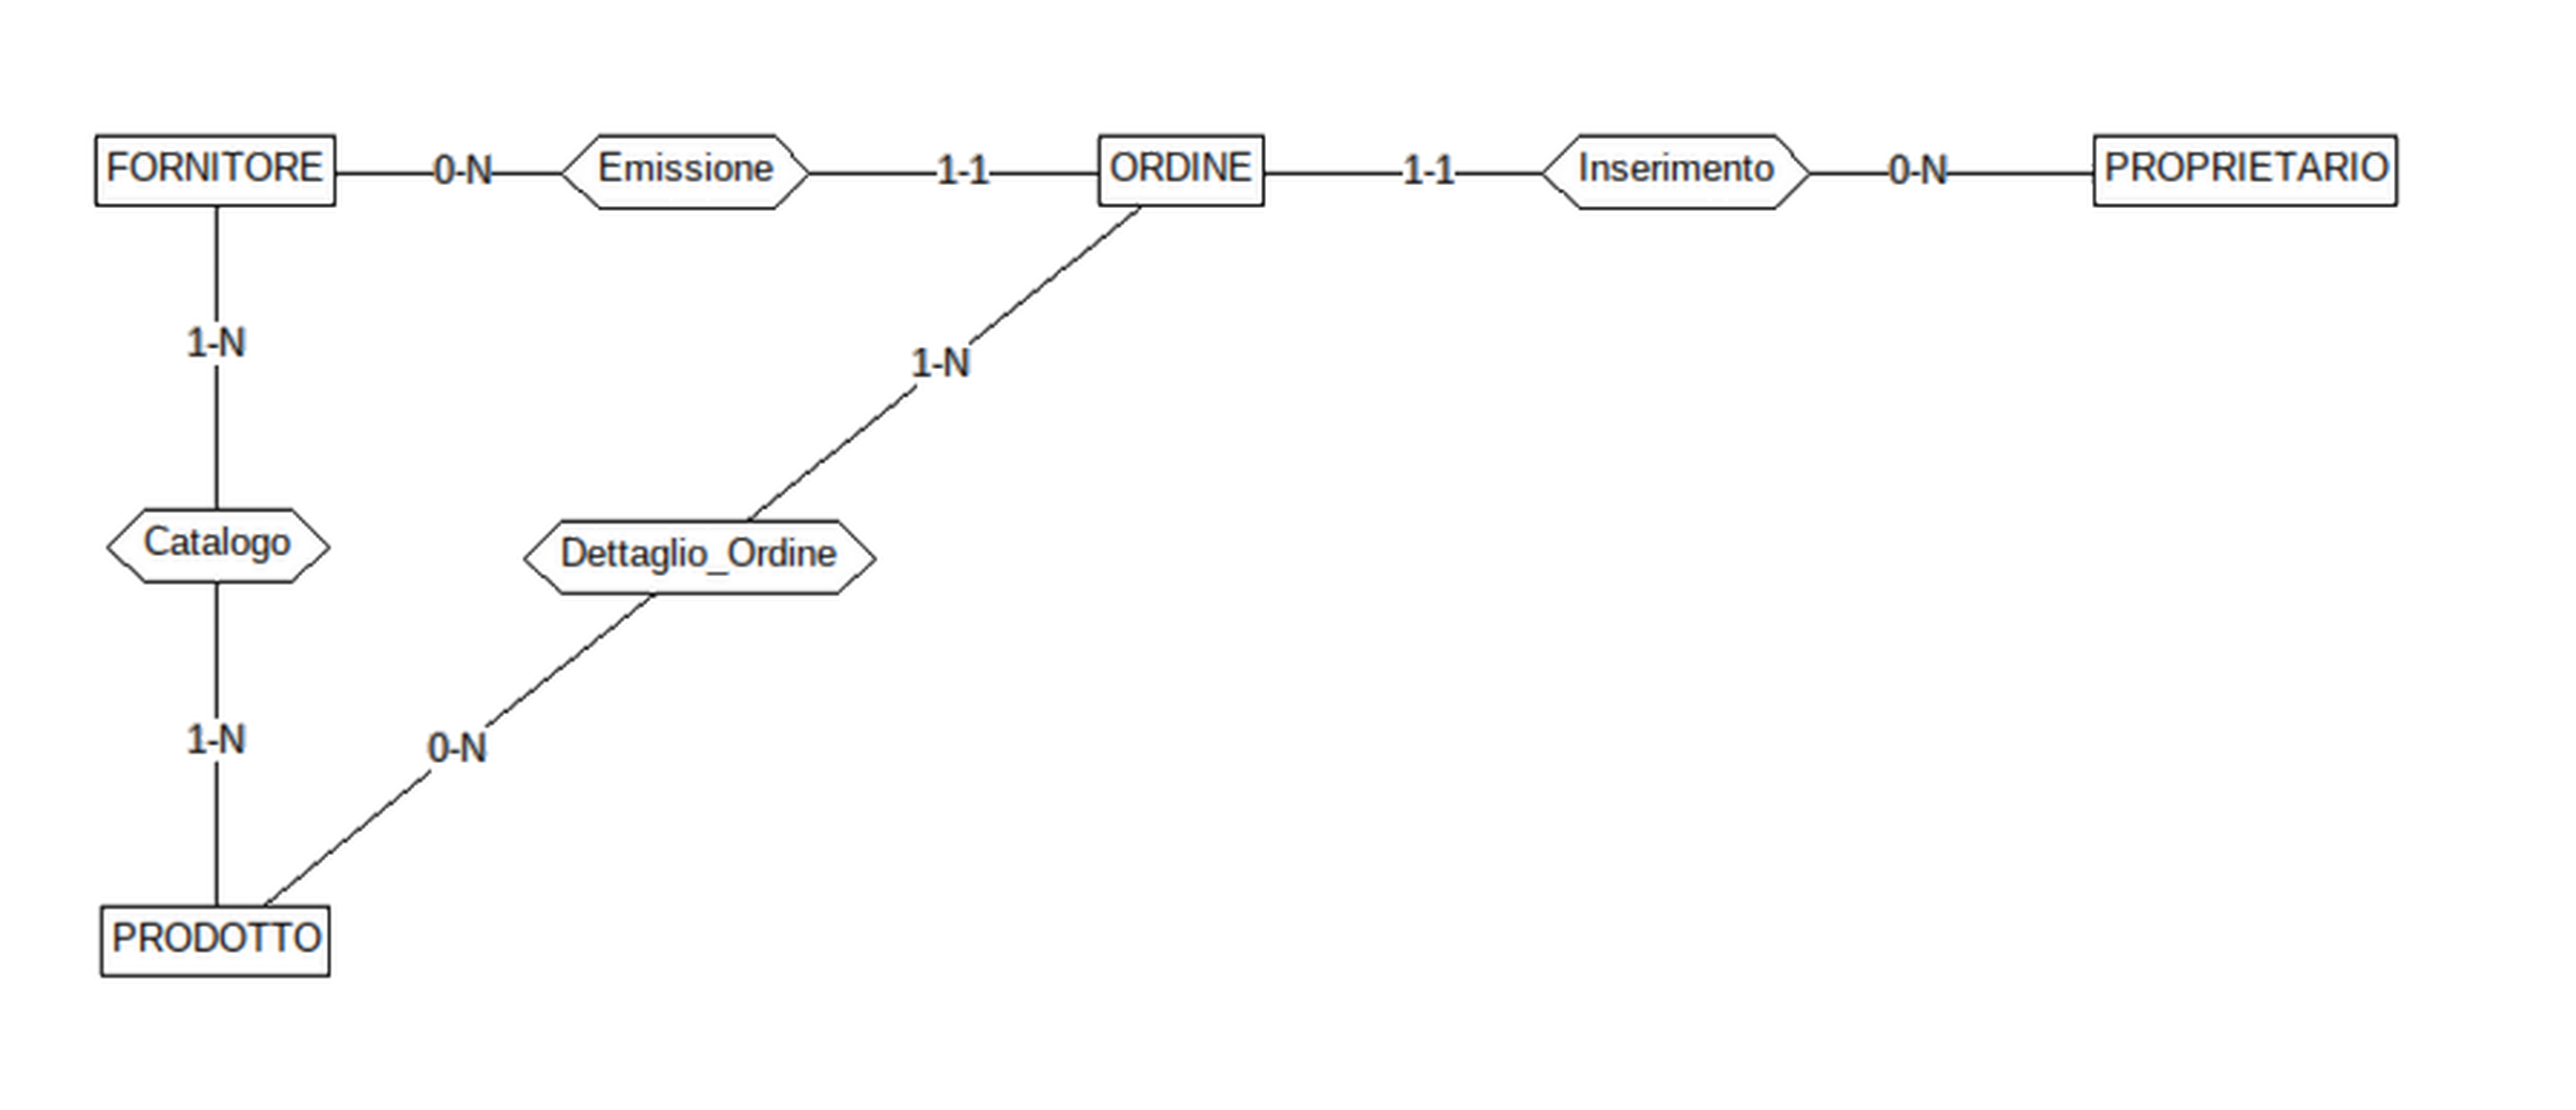
\includegraphics[width=0.9\textwidth]{immagini/03/scheletroOrdini.png}
  \caption{Schema scheletro dell'area ordini}
  \label{fig:scheletroOrdini}
\end{figure}

\subsection{Raffinamenti proposti}
\begin{itemize}
  \item L'entita \entita{Proprietario} è una specializzazione del concetto più generale di persona. Verrà
        quindi aggiunta l'entità \entita{Persona} come generalizzazione.
  \item Per ogni prodotto va memorizzata la categoria ma poiché le categorie saranno poche e molto ripetute
        è opportuna la creazione di un entità \entita{Categoria} che sara in associazione 1 a N con
        l'entità \entita{Prodotto}
  \item Il \entita{Catalogo} è meglio rappresentato da un entità così da poter garantire l'esistenza della corrispondenza tra
        prodotto e fornitore quando viene effettuato un ordine.
  \item L'entità \entita{Ordine} non sarà più associata a prodotto ma alla nuova \entita{Catalogo} così da poter
        distinguere prodotti uguali da fornitori diversi
\end{itemize}

\subsection{Schema completo}
\begin{figure}[H]
  \centering
  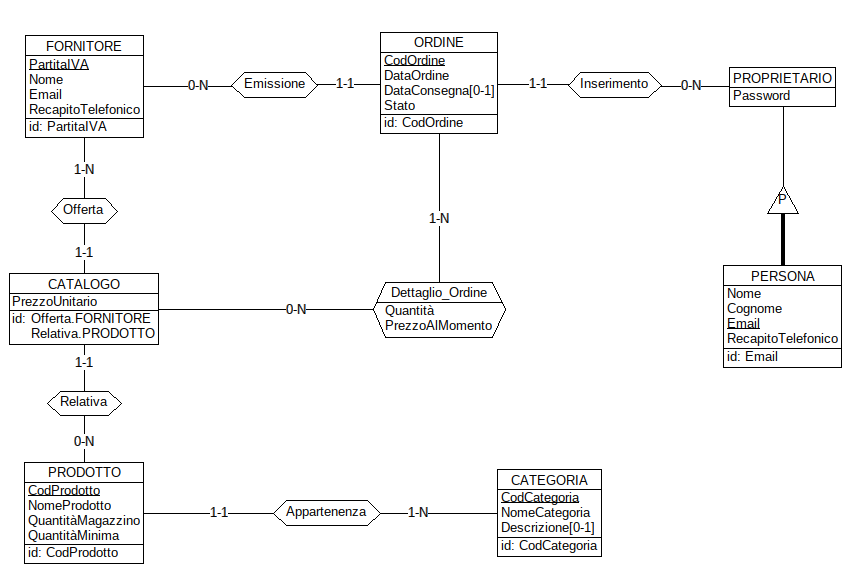
\includegraphics[width=0.9\textwidth]{immagini/03/schemaOrdiniCompleto.png}
  \caption{Schema scheletro dell'area ordini}
  \label{fig:OrdiniCompleto}
\end{figure}

\begin{notabox}[Vincolo inespresso]
Come indicato nelle specifiche un ordine può essere effettuato solo verso un unico fornitore
quindi un vincolo inespresso è che tutte le tuple di catalogo associate ad un ordine
devono avere come fornitore lo stesso dell'ordine.
\end{notabox}

\section{Area Dipendenti} % SCHEMA DA FARE

\subsection{Schema Scheletro}
\begin{figure}[H]
  \centering
  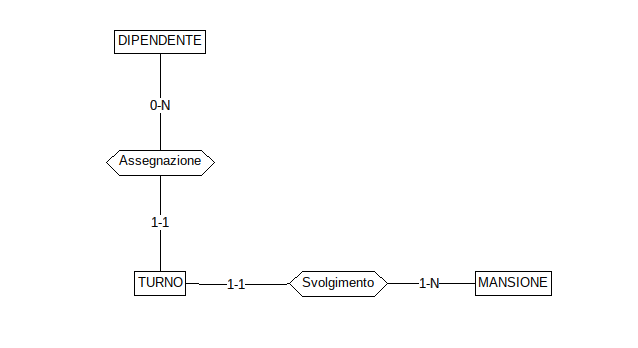
\includegraphics[width=0.9\textwidth]{immagini/03/scheletroDipendenti.png}
  \caption{Schema scheletro dell'area dipendenti e turni}
  \label{fig:scheletroDipendenti}
\end{figure}

\subsection{Raffinamenti proposti}
\begin{itemize}
  \item L'entita \entita{Dipendente} è una specializzazione del concetto più generale di persona. Verrà
        quindi aggiunta l'entità \entita{Persona} come generalizzazione.
  \item Per ogni \entita{Dipendente} va memorizzato, come informazione personale, il codice fiscale.
  \item Ogni turno sarà identificato dal lavoratore, dalla data e dall'ora d'inizio dello stesso. Per 
        questo motivo si è deciso di identificarlo con attributo composto \textit{Dipendente,Data,OraInizio},
        in modo da permettere lo svolgimento di turni \textit{spezzati}.
\end{itemize}

\begin{notabox}[Vincolo implicito]
Un dipendente non pu\`{o} lavorare, durante un turno, due volte per due lassi di tempo sovrapposti. 
Questo vincolo non \`{e} esprimibile nello schema E/R ma verr\`{a} implementato tramite
\texttt{CHECK} o trigger nel database.
\end{notabox}

\subsection{Schema completo}
\begin{figure}[H]
  \centering
  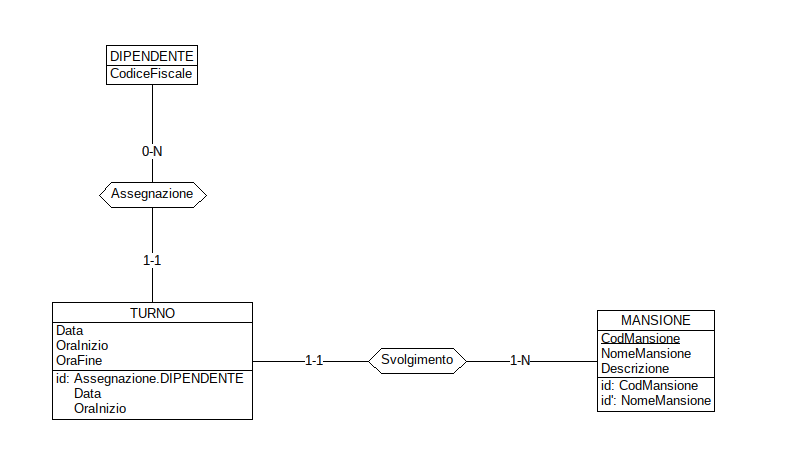
\includegraphics[width=0.9\textwidth]{immagini/03/schemaCompletoDipendenti.png}
  \caption{Schema completo dell'area dipendenti e turni}
  \label{fig:schemaDipendenti}
\end{figure}

\section{Area Spiaggia}

\subsection{Schema Scheletro} % DA FARE
\begin{figure}[H]
  \centering
  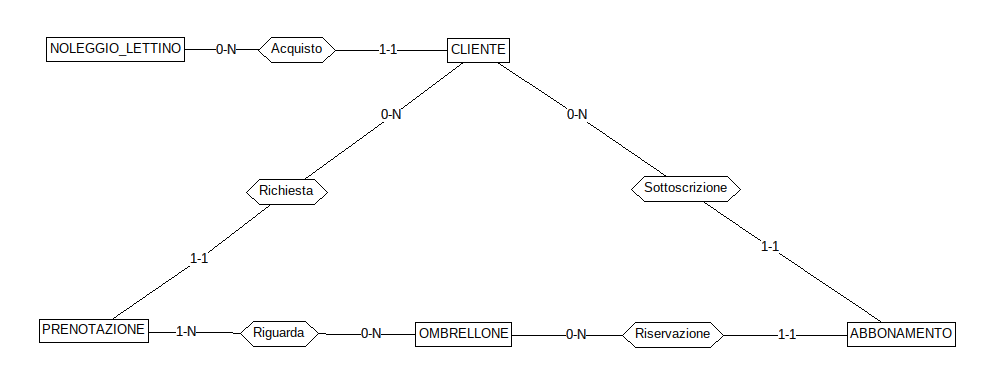
\includegraphics[width=0.9\textwidth]{immagini/03/scheletroLettiniOmbrelloni.png}
  \caption{Schema scheletro dell'area spiaggia}
  \label{fig:scheletroSpiaggia}
\end{figure}

\subsection{Raffinamenti Proposti}
\begin{itemize}
  \item L'entita \entita{Cliente} è una specializzazione del concetto più generale di persona. Verrà
        quindi aggiunta l'entità \entita{Persona} come generalizzazione.
  \item Il prezzo di un singolo noleggio
\end{itemize}

\begin{notabox}[Vincolo implicito]
Un ombrellone non pu\`{o} essere prenotato due volte per lo stesso periodo. Questo
vincolo non \`{e} esprimibile nello schema E/R ma verr\`{a} implementato tramite
\texttt{CHECK} o trigger nel database.
\end{notabox}

\subsection{Area: Ombrelloni}

\textbf{Decisione:} l'attributo \textit{posizione} viene decomposto in
\attributo{fila} (lettera, es. A--Z) e \attributo{numero} (intero progressivo).
La coppia (fila, numero) costituisce l'identificatore naturale dell'ombrellone.

\textbf{Decisione:} \attributo{numeroLettini} e \attributo{numeroSedie} rimangono
attributi dell'entit\`{a} \entita{Ombrellone} e non diventano entit\`{a} separate, in
quanto non hanno attributi propri rilevanti ai fini del sistema.

\subsection{Area: Magazzino, Prodotti e Ordini}

\textbf{Decisione:} si introduce l'associazione \relazione{Contiene} tra
\entita{Ordine} e \entita{Prodotto} con l'attributo \attributo{quantit\`{a}Ordinata}.
Questa associazione permette di gestire ordini multi-prodotto.

\textbf{Decisione:} l'attributo \attributo{quantit\`{a}} di \entita{Prodotto}
rappresenta la giacenza attuale in magazzino. Quando un ordine viene confermato,
la quantit\`{a} viene aggiornata automaticamente (trigger).

% -- 3.3 Schema concettuale finale ---------------------------
\section{Schema concettuale finale}

Di seguito si presenta lo schema E/R completo con tutti gli attributi, le
cardinalit\`{a} e i vincoli di partecipazione.

\begin{figure}[H]
  \centering
  % \includegraphics[width=\textwidth]{immagini/schema_er_finale.png}
  \fbox{\parbox{0.95\textwidth}{\centering\vspace{4cm}
    \textit{[Inserire immagine: schema\_er\_finale.png]}\\
    Schema E/R completo con attributi e cardinalit\`{a}
  \vspace{4cm}}}
  \caption{Schema E/R finale}
  \label{fig:schema-er-finale}
\end{figure}

\subsection{Tabella delle entit\`{a} e associazioni}

\begin{longtable}{L{3.5cm} C{2cm} L{8cm}}
  \caption{Entit\`{a} e associazioni dello schema concettuale finale}
  \label{tab:entita-associazioni} \\
  \toprule
  \rowcolor{primary!15}
  \textbf{Nome} & \textbf{Tipo} & \textbf{Descrizione} \\
  \midrule
  \endfirsthead
  \toprule
  \rowcolor{primary!15}
  \textbf{Nome} & \textbf{Tipo} & \textbf{Descrizione} \\
  \midrule
  \endhead
  \bottomrule
  \endfoot

  \entita{Proprietario}   & E & Utente del gestionale con accesso tramite credenziali \\
  \entita{Cliente}        & E & Persona registrata nel sistema \\
  \entita{Ombrellone}     & E & Postazione identificata da fila e numero \\
  \entita{Prenotazione}   & E & Associazione temporanea cliente--ombrellone con date \\
  \entita{Abbonamento}    & E & Contratto stagionale cliente--ombrellone \\
  \entita{Dipendente}     & E & Lavoratore dello stabilimento \\
  \entita{Turno}          & E & Fascia oraria lavorativa di un dipendente \\
  \entita{Prodotto}       & E & Articolo presente in magazzino \\
  \entita{Fornitore}      & E & Azienda da cui si acquistano prodotti \\
  \entita{Ordine}         & E & Richiesta di acquisto verso un fornitore \\
  \relazione{Effettua}    & A & Proprietario $\to$ Ordine \card{1}{N} \\
  \relazione{PrenotaOmb}  & A & Cliente $\leftrightarrow$ Ombrellone tramite Prenotazione \\
  \relazione{SottoscriAbb}& A & Cliente $\leftrightarrow$ Ombrellone tramite Abbonamento \\
  \relazione{LavoraIn}    & A & Dipendente $\to$ Turno \card{1}{N} \\
  \relazione{Rifornisce}  & A & Fornitore $\to$ Ordine \card{1}{N} \\
  \relazione{Contiene}    & A & Ordine $\leftrightarrow$ Prodotto (con quantit\`{a}) \card{N}{M} \\
  \relazione{Registra}    & A & Proprietario $\to$ Dipendente \card{1}{N} \\
  \relazione{Inserisce}   & A & Proprietario $\to$ Cliente \card{1}{N} \\
\end{longtable}
